% Options for packages loaded elsewhere
\PassOptionsToPackage{unicode}{hyperref}
\PassOptionsToPackage{hyphens}{url}
%
\documentclass[
]{article}
\usepackage{amsmath,amssymb}
\usepackage{iftex}
\ifPDFTeX
  \usepackage[T1]{fontenc}
  \usepackage[utf8]{inputenc}
  \usepackage{textcomp} % provide euro and other symbols
\else % if luatex or xetex
  \usepackage{unicode-math} % this also loads fontspec
  \defaultfontfeatures{Scale=MatchLowercase}
  \defaultfontfeatures[\rmfamily]{Ligatures=TeX,Scale=1}
\fi
\usepackage{lmodern}
\ifPDFTeX\else
  % xetex/luatex font selection
\fi
% Use upquote if available, for straight quotes in verbatim environments
\IfFileExists{upquote.sty}{\usepackage{upquote}}{}
\IfFileExists{microtype.sty}{% use microtype if available
  \usepackage[]{microtype}
  \UseMicrotypeSet[protrusion]{basicmath} % disable protrusion for tt fonts
}{}
\makeatletter
\@ifundefined{KOMAClassName}{% if non-KOMA class
  \IfFileExists{parskip.sty}{%
    \usepackage{parskip}
  }{% else
    \setlength{\parindent}{0pt}
    \setlength{\parskip}{6pt plus 2pt minus 1pt}}
}{% if KOMA class
  \KOMAoptions{parskip=half}}
\makeatother
\usepackage{xcolor}
\usepackage[margin=1in]{geometry}
\usepackage{color}
\usepackage{fancyvrb}
\newcommand{\VerbBar}{|}
\newcommand{\VERB}{\Verb[commandchars=\\\{\}]}
\DefineVerbatimEnvironment{Highlighting}{Verbatim}{commandchars=\\\{\}}
% Add ',fontsize=\small' for more characters per line
\usepackage{framed}
\definecolor{shadecolor}{RGB}{248,248,248}
\newenvironment{Shaded}{\begin{snugshade}}{\end{snugshade}}
\newcommand{\AlertTok}[1]{\textcolor[rgb]{0.94,0.16,0.16}{#1}}
\newcommand{\AnnotationTok}[1]{\textcolor[rgb]{0.56,0.35,0.01}{\textbf{\textit{#1}}}}
\newcommand{\AttributeTok}[1]{\textcolor[rgb]{0.13,0.29,0.53}{#1}}
\newcommand{\BaseNTok}[1]{\textcolor[rgb]{0.00,0.00,0.81}{#1}}
\newcommand{\BuiltInTok}[1]{#1}
\newcommand{\CharTok}[1]{\textcolor[rgb]{0.31,0.60,0.02}{#1}}
\newcommand{\CommentTok}[1]{\textcolor[rgb]{0.56,0.35,0.01}{\textit{#1}}}
\newcommand{\CommentVarTok}[1]{\textcolor[rgb]{0.56,0.35,0.01}{\textbf{\textit{#1}}}}
\newcommand{\ConstantTok}[1]{\textcolor[rgb]{0.56,0.35,0.01}{#1}}
\newcommand{\ControlFlowTok}[1]{\textcolor[rgb]{0.13,0.29,0.53}{\textbf{#1}}}
\newcommand{\DataTypeTok}[1]{\textcolor[rgb]{0.13,0.29,0.53}{#1}}
\newcommand{\DecValTok}[1]{\textcolor[rgb]{0.00,0.00,0.81}{#1}}
\newcommand{\DocumentationTok}[1]{\textcolor[rgb]{0.56,0.35,0.01}{\textbf{\textit{#1}}}}
\newcommand{\ErrorTok}[1]{\textcolor[rgb]{0.64,0.00,0.00}{\textbf{#1}}}
\newcommand{\ExtensionTok}[1]{#1}
\newcommand{\FloatTok}[1]{\textcolor[rgb]{0.00,0.00,0.81}{#1}}
\newcommand{\FunctionTok}[1]{\textcolor[rgb]{0.13,0.29,0.53}{\textbf{#1}}}
\newcommand{\ImportTok}[1]{#1}
\newcommand{\InformationTok}[1]{\textcolor[rgb]{0.56,0.35,0.01}{\textbf{\textit{#1}}}}
\newcommand{\KeywordTok}[1]{\textcolor[rgb]{0.13,0.29,0.53}{\textbf{#1}}}
\newcommand{\NormalTok}[1]{#1}
\newcommand{\OperatorTok}[1]{\textcolor[rgb]{0.81,0.36,0.00}{\textbf{#1}}}
\newcommand{\OtherTok}[1]{\textcolor[rgb]{0.56,0.35,0.01}{#1}}
\newcommand{\PreprocessorTok}[1]{\textcolor[rgb]{0.56,0.35,0.01}{\textit{#1}}}
\newcommand{\RegionMarkerTok}[1]{#1}
\newcommand{\SpecialCharTok}[1]{\textcolor[rgb]{0.81,0.36,0.00}{\textbf{#1}}}
\newcommand{\SpecialStringTok}[1]{\textcolor[rgb]{0.31,0.60,0.02}{#1}}
\newcommand{\StringTok}[1]{\textcolor[rgb]{0.31,0.60,0.02}{#1}}
\newcommand{\VariableTok}[1]{\textcolor[rgb]{0.00,0.00,0.00}{#1}}
\newcommand{\VerbatimStringTok}[1]{\textcolor[rgb]{0.31,0.60,0.02}{#1}}
\newcommand{\WarningTok}[1]{\textcolor[rgb]{0.56,0.35,0.01}{\textbf{\textit{#1}}}}
\usepackage{graphicx}
\makeatletter
\def\maxwidth{\ifdim\Gin@nat@width>\linewidth\linewidth\else\Gin@nat@width\fi}
\def\maxheight{\ifdim\Gin@nat@height>\textheight\textheight\else\Gin@nat@height\fi}
\makeatother
% Scale images if necessary, so that they will not overflow the page
% margins by default, and it is still possible to overwrite the defaults
% using explicit options in \includegraphics[width, height, ...]{}
\setkeys{Gin}{width=\maxwidth,height=\maxheight,keepaspectratio}
% Set default figure placement to htbp
\makeatletter
\def\fps@figure{htbp}
\makeatother
\setlength{\emergencystretch}{3em} % prevent overfull lines
\providecommand{\tightlist}{%
  \setlength{\itemsep}{0pt}\setlength{\parskip}{0pt}}
\setcounter{secnumdepth}{-\maxdimen} % remove section numbering
\ifLuaTeX
  \usepackage{selnolig}  % disable illegal ligatures
\fi
\IfFileExists{bookmark.sty}{\usepackage{bookmark}}{\usepackage{hyperref}}
\IfFileExists{xurl.sty}{\usepackage{xurl}}{} % add URL line breaks if available
\urlstyle{same}
\hypersetup{
  pdftitle={REM},
  hidelinks,
  pdfcreator={LaTeX via pandoc}}

\title{REM}
\author{}
\date{\vspace{-2.5em}}

\begin{document}
\maketitle

\hypertarget{interactions-and-actors-data}{%
\subsection{Interactions and Actors
Data}\label{interactions-and-actors-data}}

Interactions between the team members for high-performance sessions:

\begin{itemize}
\item
  sender
\item
  receiver
\item
  time of the interaction
\item
  type of interaction (dialogue act type)
\end{itemize}

Actors Data:

\begin{itemize}
\item
  name
\item
  gender
\end{itemize}

\begin{Shaded}
\begin{Highlighting}[]
\CommentTok{\# Interactions Data Frame (Edges)}
\NormalTok{high\_perf\_interactions }\OtherTok{\textless{}{-}} \FunctionTok{readRDS}\NormalTok{(}\StringTok{"data/high\_performance\_sessions.RData"}\NormalTok{) }\SpecialCharTok{\%\textgreater{}\%} 
  \FunctionTok{select}\NormalTok{(session, sender\_id, receiver\_id, dialog, time)}


\NormalTok{interactions }\OtherTok{\textless{}{-}}\NormalTok{ high\_perf\_interactions }\SpecialCharTok{\%\textgreater{}\%}
  \FunctionTok{mutate}\NormalTok{(}
    \AttributeTok{sender\_id =} \FunctionTok{as.integer}\NormalTok{(sender\_id),  }
    \AttributeTok{receiver\_id =} \FunctionTok{as.integer}\NormalTok{(receiver\_id), }
    \AttributeTok{dialog =} \FunctionTok{as.factor}\NormalTok{(dialog) }
\NormalTok{  )}



\NormalTok{actors\_attributes }\OtherTok{\textless{}{-}} \FunctionTok{data.frame}\NormalTok{(}
  \AttributeTok{id =} \DecValTok{1}\SpecialCharTok{:}\DecValTok{8}\NormalTok{,}
  \AttributeTok{name =} \FunctionTok{c}\NormalTok{(}\StringTok{"Igor"}\NormalTok{, }\StringTok{"Ashley"}\NormalTok{, }\StringTok{"Will"}\NormalTok{, }\StringTok{"Katya"}\NormalTok{, }\StringTok{"Saleh"}\NormalTok{, }\StringTok{"Oleg"}\NormalTok{, }\StringTok{"Vika"}\NormalTok{, }\StringTok{"Alex"}\NormalTok{),}
  \AttributeTok{gender =} \FunctionTok{c}\NormalTok{(}\StringTok{"male"}\NormalTok{, }\StringTok{"female"}\NormalTok{, }\StringTok{"male"}\NormalTok{, }\StringTok{"female"}\NormalTok{, }\StringTok{"male"}\NormalTok{, }\StringTok{"male"}\NormalTok{, }\StringTok{"female"}\NormalTok{, }\StringTok{"male"}\NormalTok{)}
\NormalTok{)}

\CommentTok{\# Create dummy variables for gender}
\NormalTok{dummyvars }\OtherTok{\textless{}{-}} \FunctionTok{dummyVars}\NormalTok{(}\StringTok{" \textasciitilde{} gender"}\NormalTok{, }\AttributeTok{data =}\NormalTok{ actors\_attributes)}
\NormalTok{actors\_attributes }\OtherTok{\textless{}{-}} \FunctionTok{cbind}\NormalTok{(actors\_attributes, }\FunctionTok{predict}\NormalTok{(dummyvars, actors\_attributes)) }\SpecialCharTok{\%\textgreater{}\%}
  \FunctionTok{select}\NormalTok{(id, name, gendermale)}
\end{Highlighting}
\end{Shaded}

\hypertarget{summary-by-session-and-speaker}{%
\subsection{Summary by Session and
Speaker}\label{summary-by-session-and-speaker}}

\begin{Shaded}
\begin{Highlighting}[]
\NormalTok{session\_dialogues }\OtherTok{\textless{}{-}}\NormalTok{ high\_perf\_interactions }\SpecialCharTok{\%\textgreater{}\%}
  \FunctionTok{group\_by}\NormalTok{(session) }\SpecialCharTok{\%\textgreater{}\%}
  \FunctionTok{summarise}\NormalTok{(}\AttributeTok{n =} \FunctionTok{n}\NormalTok{())}


\FunctionTok{ggplot}\NormalTok{(session\_dialogues, }\FunctionTok{aes}\NormalTok{(}\AttributeTok{x =} \FunctionTok{factor}\NormalTok{(session), }\AttributeTok{y =}\NormalTok{ n, }\AttributeTok{fill =} \FunctionTok{factor}\NormalTok{(session))) }\SpecialCharTok{+} 
  \FunctionTok{geom\_bar}\NormalTok{(}\AttributeTok{stat =} \StringTok{"identity"}\NormalTok{) }\SpecialCharTok{+}
  \FunctionTok{scale\_fill\_brewer}\NormalTok{(}\AttributeTok{palette =} \StringTok{"Pastel1"}\NormalTok{) }\SpecialCharTok{+}  
  \FunctionTok{labs}\NormalTok{(}\AttributeTok{title =} \StringTok{"Number of Dialogues Per Session (High Performance)"}\NormalTok{,}
       \AttributeTok{x =} \StringTok{"Session"}\NormalTok{,}
       \AttributeTok{y =} \StringTok{"Number of Dialogues"}\NormalTok{,}
       \AttributeTok{fill =} \StringTok{"Session"}\NormalTok{) }\SpecialCharTok{+}
  \FunctionTok{theme\_minimal}\NormalTok{() }\SpecialCharTok{+} 
  \FunctionTok{theme}\NormalTok{(}\AttributeTok{legend.position =} \StringTok{"none"}\NormalTok{) }
\end{Highlighting}
\end{Shaded}

\begin{center}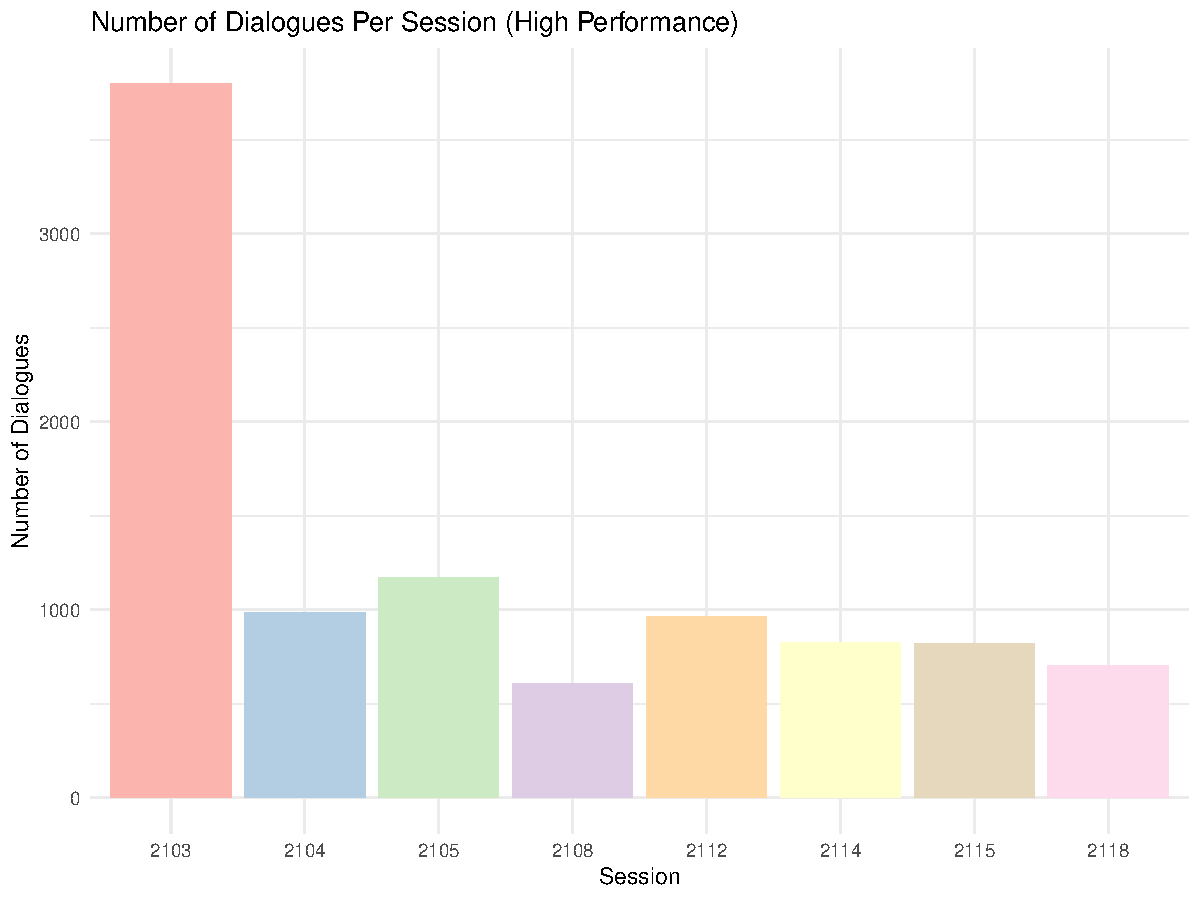
\includegraphics{april_files/figure-latex/unnamed-chunk-2-1} \end{center}

\begin{Shaded}
\begin{Highlighting}[]
\NormalTok{dialogues\_per\_speaker\_session }\OtherTok{\textless{}{-}}\NormalTok{ high\_perf\_interactions }\SpecialCharTok{\%\textgreater{}\%}
  \FunctionTok{left\_join}\NormalTok{(actors\_attributes, }\AttributeTok{by =} \FunctionTok{c}\NormalTok{(}\StringTok{"sender\_id"} \OtherTok{=} \StringTok{"id"}\NormalTok{)) }\SpecialCharTok{\%\textgreater{}\%}
  \FunctionTok{group\_by}\NormalTok{(session, name) }\SpecialCharTok{\%\textgreater{}\%}
  \FunctionTok{summarise}\NormalTok{(}\AttributeTok{number\_of\_dialogues =} \FunctionTok{n}\NormalTok{(), }\AttributeTok{.groups =} \StringTok{\textquotesingle{}drop\textquotesingle{}}\NormalTok{) }\SpecialCharTok{\%\textgreater{}\%}
  \FunctionTok{arrange}\NormalTok{(session, }\FunctionTok{desc}\NormalTok{(number\_of\_dialogues))}

\NormalTok{dialogues\_summary\_tibble }\OtherTok{\textless{}{-}} \FunctionTok{as\_tibble}\NormalTok{(dialogues\_per\_speaker\_session)}
\FunctionTok{print}\NormalTok{(dialogues\_summary\_tibble)}
\end{Highlighting}
\end{Shaded}

\begin{verbatim}
## # A tibble: 42 x 3
##    session name   number_of_dialogues
##      <dbl> <chr>                <int>
##  1    2103 Will                   830
##  2    2103 Ashley                 744
##  3    2103 Vika                   649
##  4    2103 Katya                  642
##  5    2103 Oleg                   576
##  6    2103 Saleh                  356
##  7    2104 Ashley                 238
##  8    2104 Oleg                   181
##  9    2104 Will                   179
## 10    2104 Vika                   153
## # i 32 more rows
\end{verbatim}

\begin{Shaded}
\begin{Highlighting}[]
\FunctionTok{ggplot}\NormalTok{(dialogues\_summary\_tibble, }\FunctionTok{aes}\NormalTok{(}\AttributeTok{x =}\NormalTok{ name, }\AttributeTok{y =}\NormalTok{ number\_of\_dialogues, }\AttributeTok{fill =}\NormalTok{ name)) }\SpecialCharTok{+} 
  \FunctionTok{geom\_bar}\NormalTok{(}\AttributeTok{stat =} \StringTok{"identity"}\NormalTok{) }\SpecialCharTok{+}
  \FunctionTok{facet\_wrap}\NormalTok{(}\SpecialCharTok{\textasciitilde{}}\NormalTok{session) }\SpecialCharTok{+}
  \FunctionTok{scale\_fill\_brewer}\NormalTok{(}\AttributeTok{palette =} \StringTok{"Pastel1"}\NormalTok{) }\SpecialCharTok{+}  
  \FunctionTok{labs}\NormalTok{(}\AttributeTok{subtitle =} \StringTok{"Number of Dialogues Per Speaker Per Session (High Performance)"}\NormalTok{,}
       \AttributeTok{x =} \StringTok{"Speaker"}\NormalTok{,}
       \AttributeTok{y =} \StringTok{"Number of Dialogues"}\NormalTok{,}
       \AttributeTok{fill =} \StringTok{"Speaker"}\NormalTok{) }\SpecialCharTok{+}
  \FunctionTok{theme\_minimal}\NormalTok{() }\SpecialCharTok{+} 
  \FunctionTok{theme}\NormalTok{(}\AttributeTok{legend.position =} \StringTok{"none"}\NormalTok{) }
\end{Highlighting}
\end{Shaded}

\begin{center}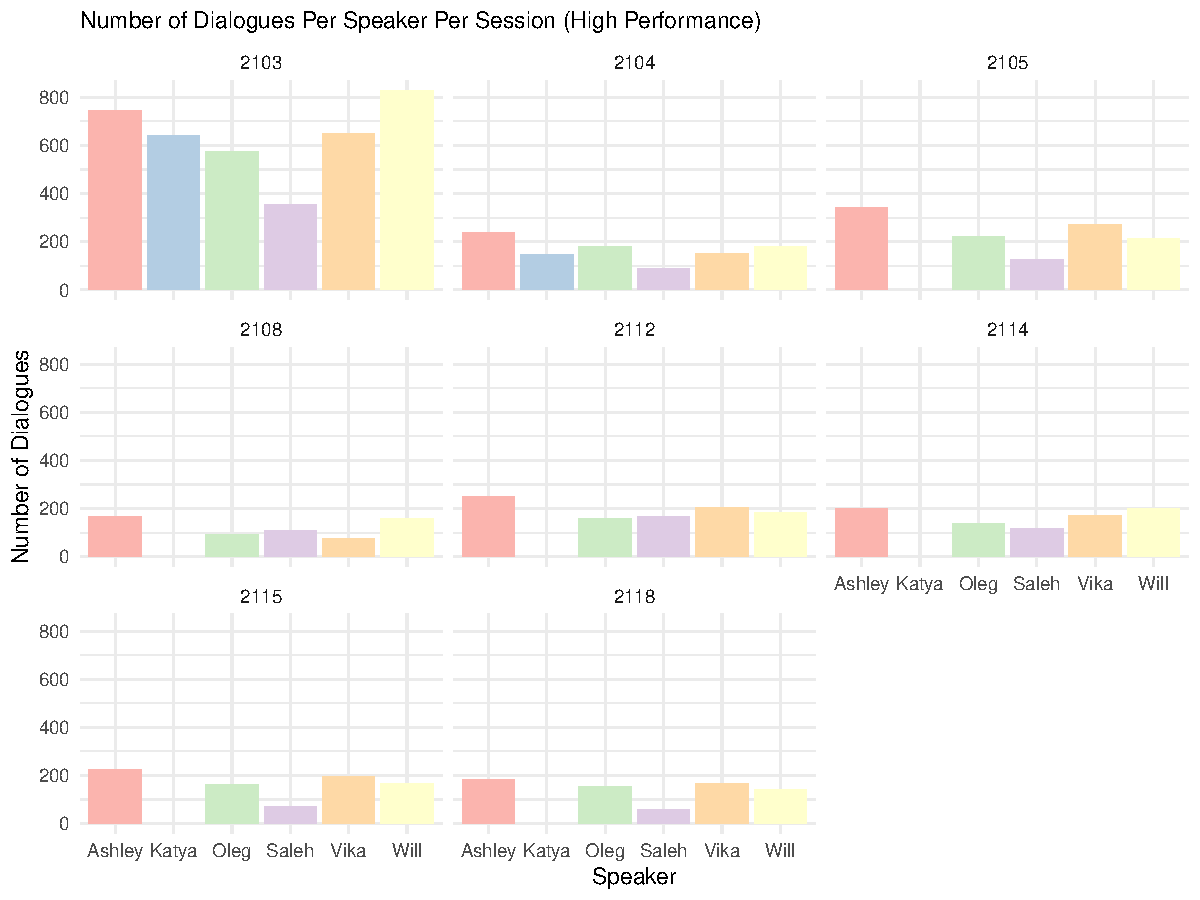
\includegraphics{april_files/figure-latex/unnamed-chunk-3-1} \end{center}

\begin{Shaded}
\begin{Highlighting}[]
\NormalTok{target\_session }\OtherTok{\textless{}{-}} \DecValTok{2104}

\NormalTok{high\_perf\_interactions }\SpecialCharTok{\%\textgreater{}\%} \FunctionTok{filter}\NormalTok{(receiver\_id }\SpecialCharTok{!=} \DecValTok{0}\NormalTok{) }\SpecialCharTok{\%\textgreater{}\%} \FunctionTok{filter}\NormalTok{(session }\SpecialCharTok{==}\NormalTok{ target\_session) }\SpecialCharTok{\%\textgreater{}\%} \FunctionTok{select}\NormalTok{(}\SpecialCharTok{{-}}\NormalTok{session) }\SpecialCharTok{\%\textgreater{}\%} \FunctionTok{mutate}\NormalTok{(}\AttributeTok{time =} \DecValTok{1}\SpecialCharTok{:}\FunctionTok{nrow}\NormalTok{(.))  }\SpecialCharTok{\%\textgreater{}\%} \FunctionTok{select}\NormalTok{(sender\_id, receiver\_id, time,dialog)  }\SpecialCharTok{\%\textgreater{}\%} \FunctionTok{mutate}\NormalTok{(}\AttributeTok{dialog =} \FunctionTok{as.factor}\NormalTok{(dialog), }\AttributeTok{sender\_id =} \FunctionTok{as.integer}\NormalTok{(sender\_id), }\AttributeTok{receiver\_id =} \FunctionTok{as.integer}\NormalTok{(receiver\_id)) }\OtherTok{{-}\textgreater{}}\NormalTok{ interactions}

\NormalTok{actors\_attributes }\SpecialCharTok{\%\textgreater{}\%} \FunctionTok{filter}\NormalTok{(id }\SpecialCharTok{\%in\%}\NormalTok{ interactions}\SpecialCharTok{$}\NormalTok{sender\_id) }\SpecialCharTok{\%\textgreater{}\%} \FunctionTok{filter}\NormalTok{(id }\SpecialCharTok{\%in\%}\NormalTok{ interactions}\SpecialCharTok{$}\NormalTok{receiver\_id) }\OtherTok{{-}\textgreater{}}\NormalTok{ actors\_attributes}
\FunctionTok{head}\NormalTok{(actors\_attributes)}
\end{Highlighting}
\end{Shaded}

\begin{verbatim}
##   id   name gendermale
## 2  2 Ashley          0
## 3  3   Will          1
## 4  4  Katya          0
## 5  5  Saleh          1
## 6  6   Oleg          1
## 7  7   Vika          0
\end{verbatim}

\begin{Shaded}
\begin{Highlighting}[]
\NormalTok{g\_subset }\OtherTok{\textless{}{-}} \FunctionTok{graph\_from\_data\_frame}\NormalTok{(interactions, }\AttributeTok{directed =} \ConstantTok{TRUE}\NormalTok{, }\AttributeTok{vertices =} \FunctionTok{data.frame}\NormalTok{(actors\_attributes))}


\FunctionTok{V}\NormalTok{(g\_subset)}\SpecialCharTok{$}\NormalTok{gender }\OtherTok{\textless{}{-}}\NormalTok{ actors\_attributes}\SpecialCharTok{$}\NormalTok{gender[}\FunctionTok{match}\NormalTok{(}\FunctionTok{V}\NormalTok{(g\_subset)}\SpecialCharTok{$}\NormalTok{name, actors\_attributes}\SpecialCharTok{$}\NormalTok{name)]}
\FunctionTok{V}\NormalTok{(g\_subset)}\SpecialCharTok{$}\NormalTok{name }\OtherTok{\textless{}{-}}\NormalTok{ actors\_attributes}\SpecialCharTok{$}\NormalTok{name[}\FunctionTok{match}\NormalTok{(}\FunctionTok{V}\NormalTok{(g\_subset)}\SpecialCharTok{$}\NormalTok{name, actors\_attributes}\SpecialCharTok{$}\NormalTok{name)]}
\end{Highlighting}
\end{Shaded}

\hypertarget{dialogue-flow-illustration}{%
\paragraph{Dialogue Flow
Illustration}\label{dialogue-flow-illustration}}

\begin{Shaded}
\begin{Highlighting}[]
\NormalTok{dialog\_colors }\OtherTok{\textless{}{-}}\NormalTok{ RColorBrewer}\SpecialCharTok{::}\FunctionTok{brewer.pal}\NormalTok{(}\AttributeTok{n =} \FunctionTok{length}\NormalTok{(}\FunctionTok{unique}\NormalTok{(interactions}\SpecialCharTok{$}\NormalTok{dialog)), }\AttributeTok{name =} \StringTok{"Pastel2"}\NormalTok{)}
\NormalTok{dialog\_color\_map }\OtherTok{\textless{}{-}} \FunctionTok{setNames}\NormalTok{(dialog\_colors, }\FunctionTok{unique}\NormalTok{(interactions}\SpecialCharTok{$}\NormalTok{dialog))}


\FunctionTok{ggraph}\NormalTok{(g\_subset, }\AttributeTok{layout =} \StringTok{\textquotesingle{}fr\textquotesingle{}}\NormalTok{) }\SpecialCharTok{+}
  \FunctionTok{geom\_edge\_link}\NormalTok{(}\FunctionTok{aes}\NormalTok{(}\AttributeTok{color =}\NormalTok{ dialog), }\AttributeTok{alpha =} \FloatTok{0.7}\NormalTok{, }\AttributeTok{edge\_width =}\NormalTok{ .}\DecValTok{2}\NormalTok{, }\AttributeTok{lineend =} \StringTok{"butt"}\NormalTok{, }\AttributeTok{arrow =} \FunctionTok{arrow}\NormalTok{(}\AttributeTok{type =} \StringTok{\textquotesingle{}closed\textquotesingle{}}\NormalTok{, }\AttributeTok{length =} \FunctionTok{unit}\NormalTok{(}\DecValTok{4}\NormalTok{, }\StringTok{\textquotesingle{}mm\textquotesingle{}}\NormalTok{))) }\SpecialCharTok{+}
  \FunctionTok{scale\_edge\_color\_manual}\NormalTok{(}\AttributeTok{values =}\NormalTok{ dialog\_color\_map) }\SpecialCharTok{+}
  \FunctionTok{geom\_node\_point}\NormalTok{(}\FunctionTok{aes}\NormalTok{(}\AttributeTok{color =} \FunctionTok{factor}\NormalTok{(gender)), }\AttributeTok{size =} \DecValTok{4}\NormalTok{, }\AttributeTok{alpha =} \FloatTok{0.8}\NormalTok{) }\SpecialCharTok{+}
  \FunctionTok{geom\_node\_text}\NormalTok{(}\FunctionTok{aes}\NormalTok{(}\AttributeTok{label =}\NormalTok{ name), }\AttributeTok{repel =} \ConstantTok{TRUE}\NormalTok{,  }\AttributeTok{color =} \StringTok{"black"}\NormalTok{, }\AttributeTok{size =} \DecValTok{3}\NormalTok{, }\AttributeTok{vjust =} \DecValTok{1}\NormalTok{, }\AttributeTok{nudge\_x =} \SpecialCharTok{{-}}\NormalTok{.}\DecValTok{02}\NormalTok{) }\SpecialCharTok{+}
  \FunctionTok{scale\_color\_manual}\NormalTok{(}\AttributeTok{values =} \FunctionTok{c}\NormalTok{(}\StringTok{\textquotesingle{}0\textquotesingle{}} \OtherTok{=} \StringTok{\textquotesingle{}red\textquotesingle{}}\NormalTok{, }\StringTok{\textquotesingle{}1\textquotesingle{}} \OtherTok{=} \StringTok{\textquotesingle{}cyan\textquotesingle{}}\NormalTok{)) }\SpecialCharTok{+}
  \FunctionTok{theme\_void}\NormalTok{() }\SpecialCharTok{+}
  \FunctionTok{labs}\NormalTok{(}\AttributeTok{subtitle =} \StringTok{"High Performing Session 2104"}\NormalTok{, }\AttributeTok{color =} \StringTok{"Gender"}\NormalTok{, }\AttributeTok{edge\_color =} \StringTok{"Dialog"}\NormalTok{) }\SpecialCharTok{+}
  \FunctionTok{theme}\NormalTok{(}\AttributeTok{legend.position =} \StringTok{"right"}\NormalTok{, }\AttributeTok{legend.title =} \FunctionTok{element\_text}\NormalTok{(}\AttributeTok{size =} \DecValTok{8}\NormalTok{))}
\end{Highlighting}
\end{Shaded}

\begin{center}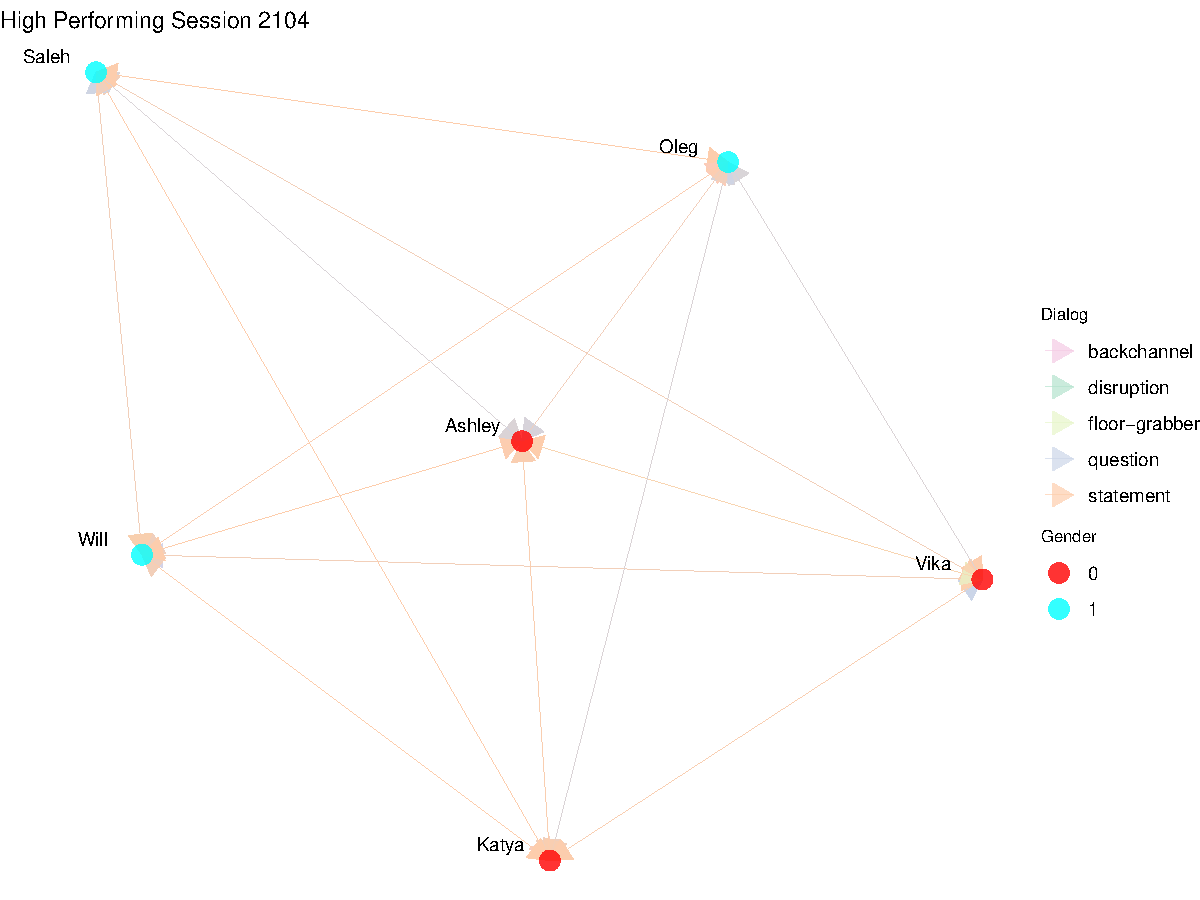
\includegraphics{april_files/figure-latex/unnamed-chunk-5-1} \end{center}

\hypertarget{degree-distribution}{%
\paragraph{Degree Distribution}\label{degree-distribution}}

\begin{Shaded}
\begin{Highlighting}[]
\NormalTok{degree\_stats }\OtherTok{\textless{}{-}} \FunctionTok{degree}\NormalTok{(g\_subset, }\AttributeTok{mode =} \StringTok{"all"}\NormalTok{)  }

\NormalTok{betweenness\_stats }\OtherTok{\textless{}{-}} \FunctionTok{betweenness}\NormalTok{(g\_subset, }\AttributeTok{directed =} \ConstantTok{TRUE}\NormalTok{)}

\NormalTok{network\_stats\_summary }\OtherTok{\textless{}{-}} \FunctionTok{data.frame}\NormalTok{(}
  \AttributeTok{name =} \FunctionTok{V}\NormalTok{(g\_subset)}\SpecialCharTok{$}\NormalTok{name,}
  \AttributeTok{degree =}\NormalTok{ degree\_stats}
\NormalTok{)}


\FunctionTok{print}\NormalTok{(network\_stats\_summary)}
\end{Highlighting}
\end{Shaded}

\begin{verbatim}
##          name degree
## Ashley Ashley    473
## Will     Will    358
## Katya   Katya    294
## Saleh   Saleh    178
## Oleg     Oleg    363
## Vika     Vika    306
\end{verbatim}

\begin{Shaded}
\begin{Highlighting}[]
\NormalTok{influencers }\OtherTok{\textless{}{-}}\NormalTok{ network\_stats\_summary }\SpecialCharTok{\%\textgreater{}\%}
  \FunctionTok{arrange}\NormalTok{(}\FunctionTok{desc}\NormalTok{(degree)) }\SpecialCharTok{\%\textgreater{}\%}
  \FunctionTok{head}\NormalTok{(}\DecValTok{3}\NormalTok{) }
\FunctionTok{print}\NormalTok{(influencers)}
\end{Highlighting}
\end{Shaded}

\begin{verbatim}
##          name degree
## Ashley Ashley    473
## Oleg     Oleg    363
## Will     Will    358
\end{verbatim}

\begin{itemize}
\item
  \textbf{Degree}: This is the number of direct connections a node has.

  \begin{itemize}
  \tightlist
  \item
    Ashley has the highest degree (473), or the greatest direct
    connections in the network.
  \end{itemize}
\item
  \textbf{Closeness}: This measures how quickly a node can access all
  other nodes in the network. Higher values represent shorter paths to
  all other nodes.

  \begin{itemize}
  \tightlist
  \item
    Ashley, with a closeness of 1.0000000, is the quickest to reach all
    other nodes.
  \end{itemize}
\end{itemize}

Check for Isolates, Connectivity, and Directionality

\begin{Shaded}
\begin{Highlighting}[]
\NormalTok{isolates }\OtherTok{\textless{}{-}} \FunctionTok{which}\NormalTok{(}\FunctionTok{degree}\NormalTok{(g\_subset) }\SpecialCharTok{==} \DecValTok{0}\NormalTok{)}
\ControlFlowTok{if}\NormalTok{ (}\FunctionTok{length}\NormalTok{(isolates) }\SpecialCharTok{\textgreater{}} \DecValTok{0}\NormalTok{) \{}
  \FunctionTok{print}\NormalTok{(}\FunctionTok{V}\NormalTok{(g\_subset)}\SpecialCharTok{$}\NormalTok{name[isolates])}
\NormalTok{\}}


\NormalTok{is.fully.connected }\OtherTok{\textless{}{-}} \FunctionTok{is\_connected}\NormalTok{(g\_subset)}
\FunctionTok{print}\NormalTok{(is.fully.connected)}
\end{Highlighting}
\end{Shaded}

\begin{verbatim}
## [1] TRUE
\end{verbatim}

\begin{Shaded}
\begin{Highlighting}[]
\NormalTok{is.directed }\OtherTok{\textless{}{-}} \FunctionTok{is\_directed}\NormalTok{(g\_subset)}
\FunctionTok{print}\NormalTok{(is.directed)}
\end{Highlighting}
\end{Shaded}

\begin{verbatim}
## [1] TRUE
\end{verbatim}

\begin{Shaded}
\begin{Highlighting}[]
\NormalTok{in\_degree\_stats }\OtherTok{\textless{}{-}} \FunctionTok{degree}\NormalTok{(g\_subset, }\AttributeTok{mode =} \StringTok{"in"}\NormalTok{)}
\NormalTok{out\_degree\_stats }\OtherTok{\textless{}{-}} \FunctionTok{degree}\NormalTok{(g\_subset, }\AttributeTok{mode =} \StringTok{"out"}\NormalTok{)}
\NormalTok{total\_degree\_stats }\OtherTok{\textless{}{-}}\NormalTok{ in\_degree\_stats }\SpecialCharTok{+}\NormalTok{ out\_degree\_stats}
\FunctionTok{rbind}\NormalTok{(in\_degree\_stats, out\_degree\_stats, total\_degree\_stats)}
\end{Highlighting}
\end{Shaded}

\begin{verbatim}
##                    Ashley Will Katya Saleh Oleg Vika
## in_degree_stats       236  179   147    89  182  153
## out_degree_stats      237  179   147    89  181  153
## total_degree_stats    473  358   294   178  363  306
\end{verbatim}

\hypertarget{rem-analysis}{%
\section{REM Analysis}\label{rem-analysis}}

\begin{Shaded}
\begin{Highlighting}[]
\NormalTok{interactions}\SpecialCharTok{$}\NormalTok{time}\OtherTok{\textless{}{-}}\FunctionTok{as.numeric}\NormalTok{(interactions}\SpecialCharTok{$}\NormalTok{time) }

\CommentTok{\# Create the REM data set}
\NormalTok{REM.data }\OtherTok{\textless{}{-}} \FunctionTok{createRemDataset}\NormalTok{(}
  \AttributeTok{data =}\NormalTok{ interactions, }
  \AttributeTok{sender =}\NormalTok{ interactions}\SpecialCharTok{$}\NormalTok{sender\_id,}
  \AttributeTok{target =}\NormalTok{ interactions}\SpecialCharTok{$}\NormalTok{receiver\_id,}
  \AttributeTok{eventSequence =}\NormalTok{ interactions}\SpecialCharTok{$}\NormalTok{time,}
  \AttributeTok{eventAttribute =}\NormalTok{ interactions}\SpecialCharTok{$}\NormalTok{dialog,}
  \AttributeTok{atEventTimesOnly =} \ConstantTok{TRUE}\NormalTok{, }
  \AttributeTok{untilEventOccurrs =} \ConstantTok{TRUE}\NormalTok{,}
  \AttributeTok{includeAllPossibleEvents =} \ConstantTok{FALSE}\NormalTok{, }
  \AttributeTok{returnInputData =} \ConstantTok{FALSE}
\NormalTok{)}

\CommentTok{\#save as RDS}
\CommentTok{\#saveRDS(REM.data, "data/REM\_data\_onlyevent.RDS")}
\end{Highlighting}
\end{Shaded}

\begin{Shaded}
\begin{Highlighting}[]
\FunctionTok{readRDS}\NormalTok{(}\StringTok{"data/REM\_data.RDS"}\NormalTok{) }\OtherTok{{-}\textgreater{}}\NormalTok{ REM.data}
\end{Highlighting}
\end{Shaded}

\begin{Shaded}
\begin{Highlighting}[]
\CommentTok{\# Check the structure of the REM.data}
\FunctionTok{str}\NormalTok{(REM.data)}
\end{Highlighting}
\end{Shaded}

\begin{verbatim}
## 'data.frame':    90290 obs. of  12 variables:
##  $ target          : chr  "2" "2" "2" "2" ...
##  $ sender          : chr  "2" "3" "3" "6" ...
##  $ eventID         : chr  "eventID1" "eventID96" "eventID96" "eventID969" ...
##  $ eventTime       : num  1 38 39 959 960 961 962 179 180 181 ...
##  $ eventDummy      : num  1 0 0 0 0 0 0 0 0 0 ...
##  $ eventAtRiskFrom : num  1 1 1 949 949 949 949 1 1 1 ...
##  $ eventAtRiskUntil: num  1 96 96 969 969 969 969 199 199 199 ...
##  $ eventAttribute  : chr  "disruption" "statement" "statement" "statement" ...
##  $ name.x          : chr  "Ashley" "Will" "Will" "Oleg" ...
##  $ gendermale.x    : num  0 1 1 1 1 1 1 0 0 0 ...
##  $ name.y          : chr  "Ashley" "Ashley" "Ashley" "Ashley" ...
##  $ gendermale.y    : num  0 0 0 0 0 0 0 0 0 0 ...
\end{verbatim}

\begin{Shaded}
\begin{Highlighting}[]
\FunctionTok{head}\NormalTok{(REM.data)}
\end{Highlighting}
\end{Shaded}

\begin{verbatim}
##   target sender    eventID eventTime eventDummy eventAtRiskFrom
## 1      2      2   eventID1         1          1               1
## 2      2      3  eventID96        38          0               1
## 3      2      3  eventID96        39          0               1
## 4      2      6 eventID969       959          0             949
## 5      2      6 eventID969       960          0             949
## 6      2      6 eventID969       961          0             949
##   eventAtRiskUntil eventAttribute name.x gendermale.x name.y gendermale.y
## 1                1     disruption Ashley            0 Ashley            0
## 2               96      statement   Will            1 Ashley            0
## 3               96      statement   Will            1 Ashley            0
## 4              969      statement   Oleg            1 Ashley            0
## 5              969      statement   Oleg            1 Ashley            0
## 6              969      statement   Oleg            1 Ashley            0
\end{verbatim}

\begin{Shaded}
\begin{Highlighting}[]
\NormalTok{surv\_object }\OtherTok{\textless{}{-}} \FunctionTok{Surv}\NormalTok{(}\AttributeTok{time =}\NormalTok{ REM.data}\SpecialCharTok{$}\NormalTok{eventTime, }\AttributeTok{event =}\NormalTok{ REM.data}\SpecialCharTok{$}\NormalTok{eventDummy)}


\NormalTok{cox\_model }\OtherTok{\textless{}{-}} \FunctionTok{coxph}\NormalTok{(surv\_object }\SpecialCharTok{\textasciitilde{}}\NormalTok{ sender }\SpecialCharTok{+}\NormalTok{ target, }\AttributeTok{data =}\NormalTok{ REM.data)}


\FunctionTok{summary}\NormalTok{(cox\_model)}
\end{Highlighting}
\end{Shaded}

\begin{verbatim}
## Call:
## coxph(formula = surv_object ~ sender + target, data = REM.data)
## 
##   n= 90290, number of events= 986 
## 
##            coef exp(coef) se(coef)      z Pr(>|z|)    
## sender3 -0.4268    0.6526   0.1033 -4.131 3.62e-05 ***
## sender4 -0.2163    0.8055   0.1072 -2.018   0.0436 *  
## sender5 -0.8191    0.4408   0.1267 -6.463 1.03e-10 ***
## sender6 -0.4809    0.6182   0.1024 -4.697 2.63e-06 ***
## sender7 -0.4295    0.6509   0.1070 -4.015 5.94e-05 ***
## target3 -0.4370    0.6460   0.1033 -4.230 2.34e-05 ***
## target4 -0.1341    0.8745   0.1077 -1.245   0.2131    
## target5 -0.7362    0.4789   0.1270 -5.798 6.72e-09 ***
## target6 -0.5767    0.5617   0.1027 -5.618 1.94e-08 ***
## target7 -0.1409    0.8686   0.1053 -1.339   0.1807    
## ---
## Signif. codes:  0 '***' 0.001 '**' 0.01 '*' 0.05 '.' 0.1 ' ' 1
## 
##         exp(coef) exp(-coef) lower .95 upper .95
## sender3    0.6526      1.532    0.5329    0.7991
## sender4    0.8055      1.241    0.6529    0.9938
## sender5    0.4408      2.268    0.3439    0.5651
## sender6    0.6182      1.618    0.5058    0.7556
## sender7    0.6509      1.536    0.5278    0.8026
## target3    0.6460      1.548    0.5275    0.7910
## target4    0.8745      1.143    0.7081    1.0800
## target5    0.4789      2.088    0.3734    0.6143
## target6    0.5617      1.780    0.4593    0.6869
## target7    0.8686      1.151    0.7067    1.0676
## 
## Concordance= 0.606  (se = 0.011 )
## Likelihood ratio test= 93.47  on 10 df,   p=1e-15
## Wald test            = 90.93  on 10 df,   p=4e-15
## Score (logrank) test = 92.43  on 10 df,   p=2e-15
\end{verbatim}

\begin{Shaded}
\begin{Highlighting}[]
\NormalTok{model2\_event }\OtherTok{\textless{}{-}} \FunctionTok{coxph}\NormalTok{(surv\_object }\SpecialCharTok{\textasciitilde{}}\NormalTok{ eventAttribute, }\AttributeTok{data =}\NormalTok{ REM.data)}
\FunctionTok{summary}\NormalTok{(model2\_event)}
\end{Highlighting}
\end{Shaded}

\begin{verbatim}
## Call:
## coxph(formula = surv_object ~ eventAttribute, data = REM.data)
## 
##   n= 90290, number of events= 986 
## 
##                               coef exp(coef) se(coef)     z Pr(>|z|)    
## eventAttributedisruption    0.1617    1.1755   0.2717 0.595    0.552    
## eventAttributefloor-grabber 0.3357    1.3989   0.2273 1.477    0.140    
## eventAttributequestion      0.9340    2.5447   0.1853 5.041 4.63e-07 ***
## eventAttributestatement     1.4839    4.4099   0.1789 8.294  < 2e-16 ***
## ---
## Signif. codes:  0 '***' 0.001 '**' 0.01 '*' 0.05 '.' 0.1 ' ' 1
## 
##                             exp(coef) exp(-coef) lower .95 upper .95
## eventAttributedisruption        1.176     0.8507    0.6901     2.002
## eventAttributefloor-grabber     1.399     0.7148    0.8961     2.184
## eventAttributequestion          2.545     0.3930    1.7698     3.659
## eventAttributestatement         4.410     0.2268    3.1056     6.262
## 
## Concordance= 0.641  (se = 0.009 )
## Likelihood ratio test= 207  on 4 df,   p=<2e-16
## Wald test            = 172.3  on 4 df,   p=<2e-16
## Score (logrank) test = 190.6  on 4 df,   p=<2e-16
\end{verbatim}

\begin{Shaded}
\begin{Highlighting}[]
\NormalTok{model3\_snd\_event }\OtherTok{\textless{}{-}} \FunctionTok{coxph}\NormalTok{(surv\_object }\SpecialCharTok{\textasciitilde{}}\NormalTok{ sender }\SpecialCharTok{+}\NormalTok{ eventAttribute, }\AttributeTok{data =}\NormalTok{ REM.data)}
\FunctionTok{summary}\NormalTok{(model3\_snd\_event)}
\end{Highlighting}
\end{Shaded}

\begin{verbatim}
## Call:
## coxph(formula = surv_object ~ sender + eventAttribute, data = REM.data)
## 
##   n= 90290, number of events= 986 
## 
##                                 coef exp(coef) se(coef)      z Pr(>|z|)    
## sender3                     -0.32011   0.72607  0.09953 -3.216 0.001299 ** 
## sender4                     -0.36260   0.69586  0.10563 -3.433 0.000598 ***
## sender5                     -0.76721   0.46431  0.12467 -6.154 7.55e-10 ***
## sender6                     -0.49032   0.61243  0.09967 -4.919 8.68e-07 ***
## sender7                     -0.32726   0.72089  0.10440 -3.135 0.001720 ** 
## eventAttributedisruption     0.23939   1.27048  0.27340  0.876 0.381237    
## eventAttributefloor-grabber  0.38767   1.47355  0.22795  1.701 0.088995 .  
## eventAttributequestion       1.04592   2.84602  0.18777  5.570 2.55e-08 ***
## eventAttributestatement      1.58097   4.85967  0.18048  8.760  < 2e-16 ***
## ---
## Signif. codes:  0 '***' 0.001 '**' 0.01 '*' 0.05 '.' 0.1 ' ' 1
## 
##                             exp(coef) exp(-coef) lower .95 upper .95
## sender3                        0.7261     1.3773    0.5974    0.8825
## sender4                        0.6959     1.4371    0.5657    0.8559
## sender5                        0.4643     2.1538    0.3637    0.5928
## sender6                        0.6124     1.6328    0.5038    0.7446
## sender7                        0.7209     1.3872    0.5875    0.8846
## eventAttributedisruption       1.2705     0.7871    0.7434    2.1711
## eventAttributefloor-grabber    1.4735     0.6786    0.9426    2.3035
## eventAttributequestion         2.8460     0.3514    1.9697    4.1122
## eventAttributestatement        4.8597     0.2058    3.4118    6.9220
## 
## Concordance= 0.665  (se = 0.01 )
## Likelihood ratio test= 254.2  on 9 df,   p=<2e-16
## Wald test            = 219.7  on 9 df,   p=<2e-16
## Score (logrank) test = 238.7  on 9 df,   p=<2e-16
\end{verbatim}

\begin{itemize}
\tightlist
\item
  The \texttt{Concordance} statistic is a measure of the model's
  predictive ability, with 0.5 indicating no predictive ability and 1
  indicating perfect prediction.
\end{itemize}

\hypertarget{survival-analysis}{%
\subsubsection{Survival Analysis}\label{survival-analysis}}

\begin{itemize}
\item
  How different factors (like senders, targets, event attributes) affect
  the likelihood of events:
\item
  \texttt{coef} in the model indicate the \emph{logarithmic} change in
  hazard rates for different categories compared to a \emph{baseline}. A
  positive coefficient indicates an increased hazard (or risk) of the
  event occurring when the variable increases, while a negative
  coefficient indicates a decreased hazard.
\item
  \texttt{exp(coef)} represents the \emph{hazard ratio}, which explains
  the effect size. values greater than 1 indicate an increased hazard,
  values less than 1 indicate a decreased hazard.
\item
  The p-values (\texttt{Pr(\textgreater{}\textbar{}z\textbar{})}) help
  determine the significance of the predictors.
\end{itemize}

\hypertarget{result-analysis}{%
\subsection{Result Analysis:}\label{result-analysis}}

\textbf{Model 1: \texttt{sender} + \texttt{target}} as predictors

predictors are the sender and target IDs of the events.

\begin{itemize}
\tightlist
\item
  \textbf{Senders 3, 4, 5, 6, and 7} have significant negative
  coefficients, suggesting that events sent by these individuals are
  less likely to occur compared to the baseline.
\item
  \textbf{Target 3 and 6} have significant negative coefficients,
  indicating events targeting these individuals are less likely to occur
  than the baseline target.
\item
  The p-values for the above mentioned actors are all below 0.05.
\item
  The overall model shows good predictive power with a concordance index
  of 0.606.
\end{itemize}

\textbf{Model 2: \texttt{eventAttribute}} as predictors

\begin{itemize}
\tightlist
\item
  \textbf{\texttt{question} and \texttt{statement} types of dialog} have
  a positive and significant effect on the hazard, indicating these
  types of events are more likely to occur. Their coefficients are
  positive with low p-values (\textless{} 2e-16 for \texttt{statement},
  4.63e-07 for \texttt{question}), showing strong evidence for their
  influence.
\item
  The \texttt{disruption} and \texttt{floor-grabber} types do not show a
  significant effect since their p-values are above 0.05.
\item
  The model has a concordance index of 0.641, indicating a reasonably
  good fit.
\end{itemize}

\textbf{Model 3: \texttt{sender} + \texttt{eventAttribute}} - senders
and dialog types as predictors.

\begin{itemize}
\tightlist
\item
  Similar to Model 1, \textbf{senders 3, 4, 5, 6, and 7} are significant
  predictors with negative coefficients, meaning events from these
  senders are less likely to happen compared to the reference sender.
\item
  As in Model 2, \textbf{\texttt{question} and \texttt{statement}} types
  of dialog are significant with positive coefficients, which means
  these event types are more likely to occur.
\item
  The coefficients for \texttt{disruption} and \texttt{floor-grabber}
  are not significant in this model as well
\item
  The concordance index is 0.665, the \textbf{highest} among the three
  models, suggesting this model has the best predictive ability.
\end{itemize}

\hypertarget{summary}{%
\subsubsection{Summary}\label{summary}}

\begin{itemize}
\tightlist
\item
  \textbf{Sender Effect}: Negative coefficients for all senders indicate
  they all decrease the event's hazard compared to a baseline, with
  \texttt{sender5} showing a significant reduction.
\item
  \textbf{Target Effect}: Similarly, most targets also reduce hazard
  rates, except \texttt{target4} and \texttt{target7} where the effect
  is not significant.
\item
  \textbf{Event Attributes} significantly increases the hazard of an
  event occurring.

  \begin{itemize}
  \tightlist
  \item
    The \texttt{eventAttribute} variables have significant coefficients
    for \texttt{question} and \texttt{statement}, indicating that these
    attributes are associated with the occurrence of events.
  \item
    The hazard ratio of \texttt{statement} is about 4.41, suggesting its
    strong association with the occurrence of events\ldots Is the effect
    of ``statement'' on event occurrences is genuinely significant, or
    is it inflated by the volume?
  \item
    \texttt{question} turns out to be important!
  \end{itemize}
\end{itemize}

\end{document}
